\chapter{Implications}
\label{chap:possible-applications}
\epigraph{``More effective tools could be built if we understood the creation process and knew what tools were needed to support human weaknesses and magnify human strengths.''}{\textit{Barbara Kitchenham}}
\noindent
This quote by Barbara Kitchenham applies to tools in general.
Speaking of tools used in software development \textcite{kitchenham_research_1990} further specify these as ``thinking tools for thinking.''
In this chapter the various ideas and findings are presented that build upon the foundation presented in \cref{chap:technological-foundation} and \cref{chap:psychological-foundation}.

As shown in \cref{sec:characteristics-of-software-development-processes} software development processes involve a lot of participants.
The customer or user imagines the perfect product, the requirements engineer thinks in user stories, testers use acceptance criteria and developers think in source code.
Each of them creates an own mental model trying to solve one part of the common problem.
Approaching a common problem with different mental representations results in the use of different tools, thus speaking ``different languages'' requiring translations or cross-domain knowledge and understanding of the people involved.

The title of this thesis promises the alignment of mental models to models used in software development.
Considering specific mental models or models used in software development and creating counterparts would solve those problems in specific cases.
Of much greater impact would be the creation of a software modelling tool that is aligned to the nature of mental models, thus enabling modelling in software development in such a way that it is analogous to developing mental models.


\section{Combining Statecharts and Hole-Driven Development}
\label{sec:combining-statecharts-and-hole-driven-development}
To the knowledge of the author, Statecharts and hole-driven-development have not yet been combined.
By integrating the concept of holes into the notation of Statecharts, the visual formalism as introduced by \textcite{harel_statecharts:_1987} is extended by the property of \emph{incompleteness}.
\cref{fig:statecharts-hole-example} exemplifies how such an extension may look like.
The goal of this thesis is not to invent a notation for such an extension.
Merely the author explains ways of how such a combination could improve the process of software development backed by psychological research.
\begin{figure}[h]
\centering
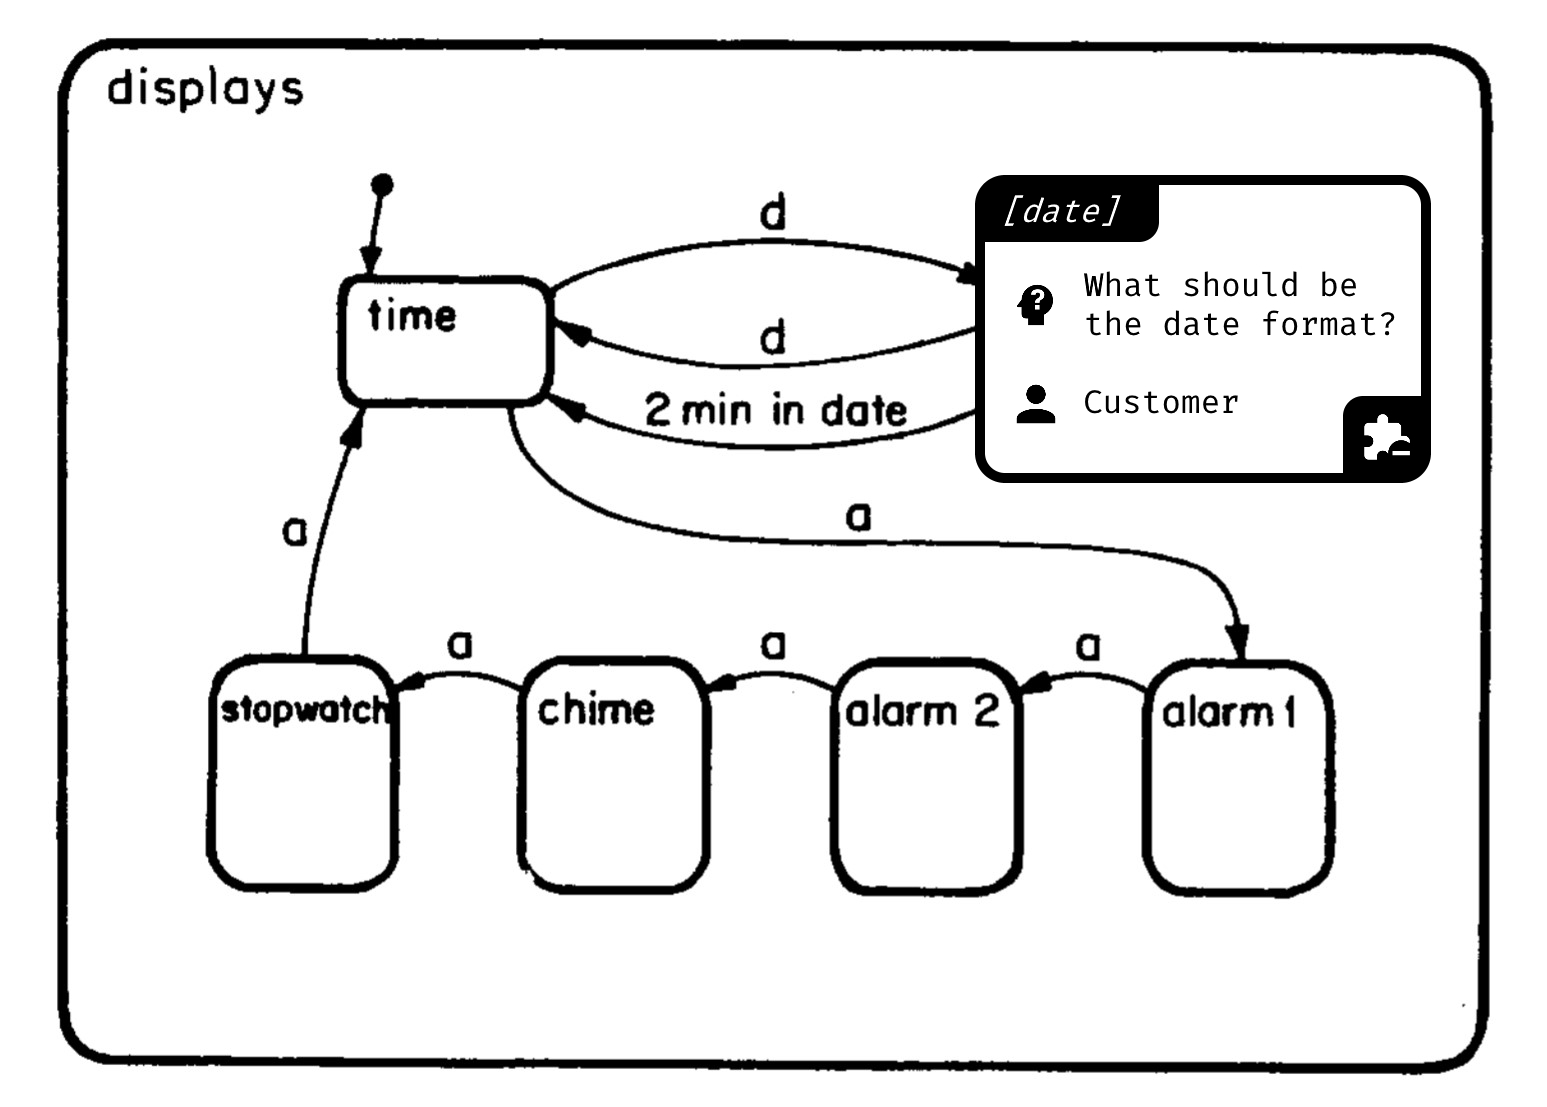
\includegraphics[width=0.8\textwidth]{images/statechart-hole-example}
\caption{Statechart including the state hole ``date''}
\label{fig:statecharts-hole-example}
\end{figure}
In comparison to \cref{fig:statecharts-example}, the state \emph{date} is now replaced by a \emph{state hole} named date, which is indicated by the icon of a missing puzzle as well as the name in brackets.
As explained in \cref{sub:hole-driven-development-in-idris} typed holes are labels that serve as questions to the compiler.
Not targeted at compilers, but at other participants in the software development process, holes in Statecharts convey way more information.
A hole without any context is useless, thus the most important information is the reason for the creation of a hole.
In this example, somebody in the software development process (probably a developer or requirements analyst) was unsure about the date format that should be used while presenting the date on the watch.
Intended as a tool simplifying communication, the role of a person intended to respond (customer in this example) is specified as well.
Summarizing this description the creator of this hole might have thought: ``I already know there should be a state called date in the behaviour of the watch, but I am unsure about the date format to display, thus I am asking the customer (or a product manager acting as the customer) for clarification.''

By combining Statecharts and hole-driven development it seems possible to
\begin{itemize}
    \item \emph{specify requirements} using a visual formalism \autocite{leveson_experiences_1991},
    \item create a \emph{shared model of understanding} (see \cref{sec:mental-models}),
    \item that can be directly \emph{executed} \autocite{harel_statecharts:_1987},
    \item \emph{aligned to the thought process} of developing software (see \cref{sub:aligning-thoughts-with-fractal-architectures}, \cref{sec:psychology-of-programming}),
    \item while \emph{improving communication} in the software development process (see \cref{sub:insights-from-psychology}).
\end{itemize}
\textcite{visser_expert_1990} 
Based on their conducted research, \textcite{visser_expert_1990} identified five rules for tools that assist the design activity.
Does the combination of Statecharts and hole-driven development adhere to these rules?


% Statecharts are just a static representation of data -> declarative programming
% during this chapter properties of mental models
% - based on beliefs, generate descriptions
% - anticipate behaviour
% - might be erroneous and incomplete
% - flexible
% - temporary
% - adapt to new information
% - capability of simulation

\subsubsection{1\textsuperscript{st} rule: assisting the management of working memory}
The cognitive system working memory acts as a buffer between the sensory register and the long-term store, its capacity is limited and information is only held temporarily \autocite{herczeg_software-ergonomie_2018}.
Regarding the performance of the working memory, $7 \pm 2$ chunks can be stored for around $15-30$ seconds \autocite{herczeg_software-ergonomie_2018}.
As presented by \textcite{victor_inventing_2012} these limitations seriously restrict the understanding and mental simulation of a program's behaviour, thus longing for interactive visual alternatives.
Based on the results of various studies \textcite{dutke_mentale_1994} states that on principle visualizations support cognitive processes, while entailing the major risk of a mental overload.
Such an example is presented in \cref{fig:full-wristwatch-statechart} \autocite{harel_modeling_1998}.
\begin{figure}[h]
\centering
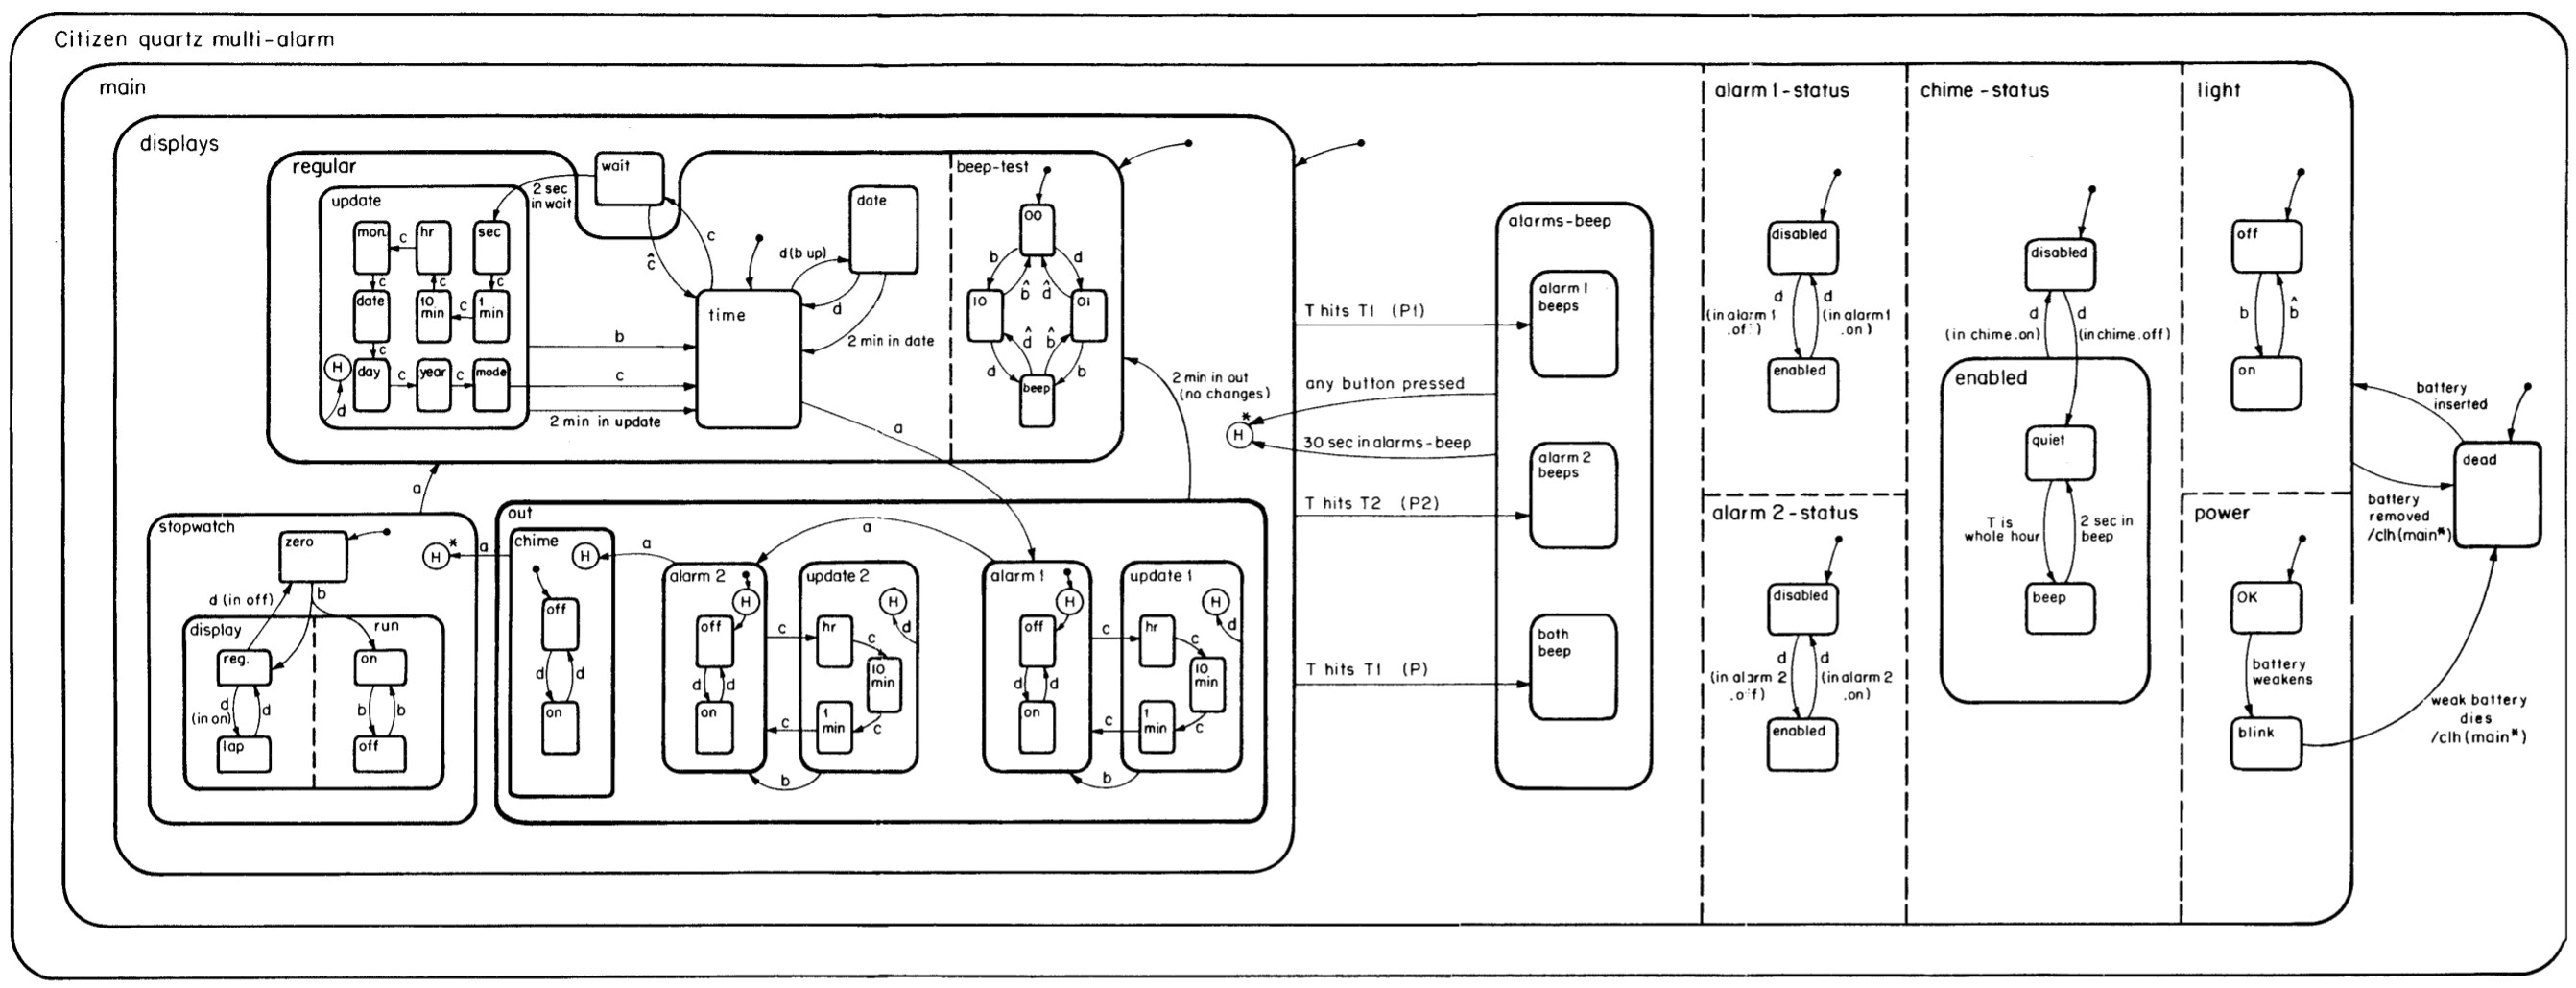
\includegraphics[width=\textwidth]{images/full-watch-statechart}
\caption{Full Statechart of a Digital Wristwatch Interface}
\label{fig:full-wristwatch-statechart}
\end{figure}
Despite the fact that the behaviour of the full system is visible at one glance, this Statechart is impractical to use in this form \autocite{harel_statecharts:_1987}.
It lost a model's character of abstraction.
For getting an overview of the full system it is not abstract enough and for understanding a certain part of the wristwatch there is too much noise \autocite{dutke_mentale_1994}.

Due to the fractal nature of Statecharts (see \cref{sub:aligning-thoughts-with-fractal-architectures}) the various sub-states can be folded away and the same model can be visualized as \cref{fig:simplified-wristwatch-statechart}.
It is important to note that the underlying model did not change, only its representation.
\begin{figure}[h]
\centering
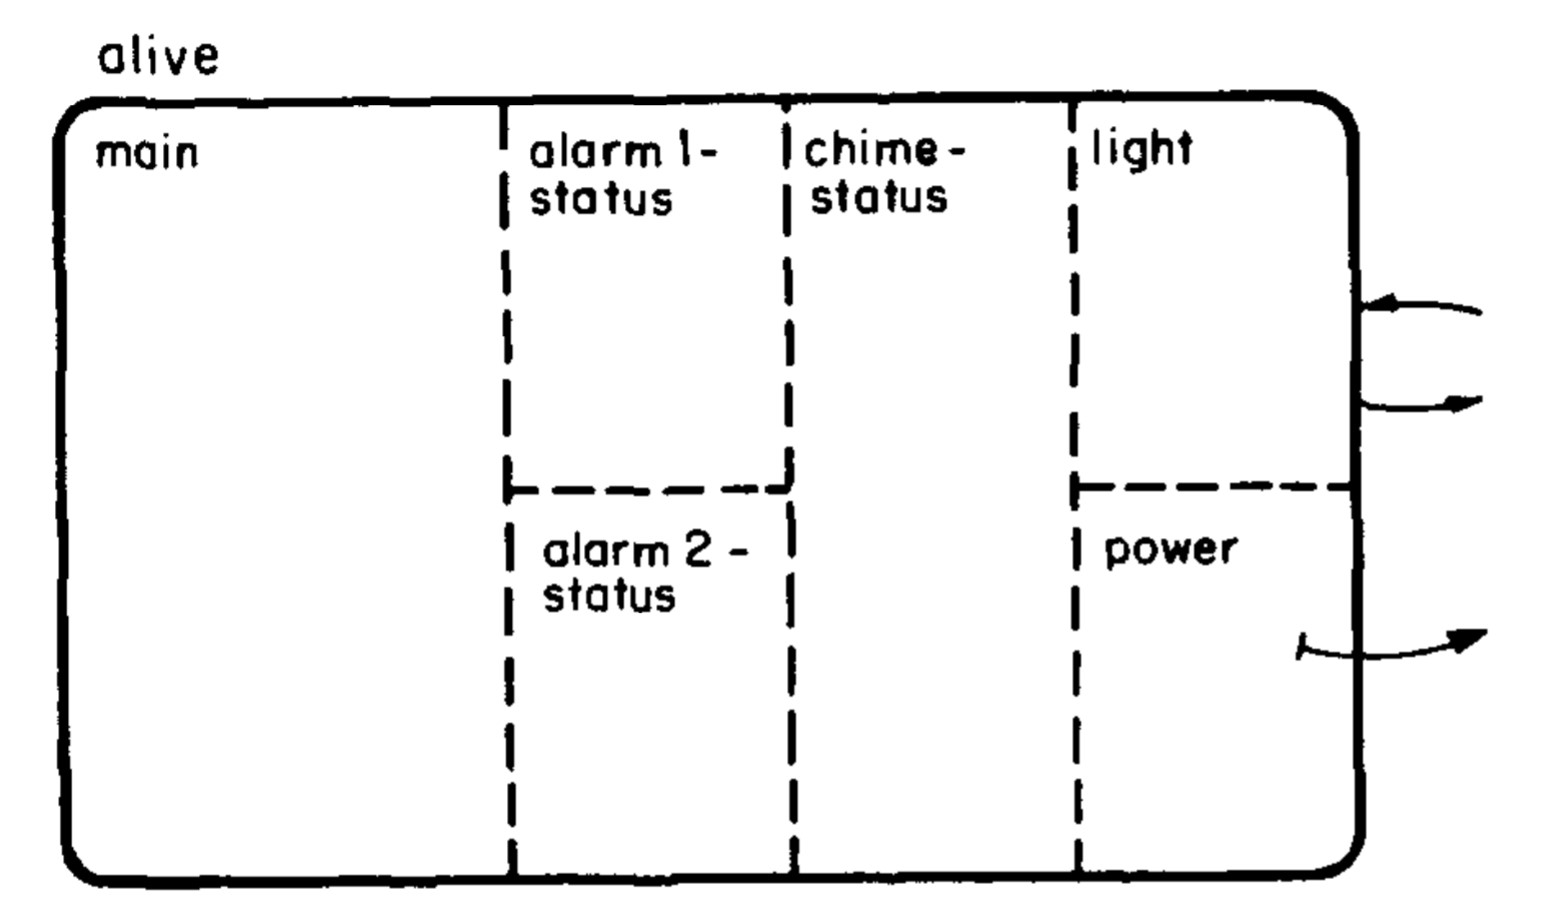
\includegraphics[width=0.8\textwidth]{images/abstract-watch-statechart}
\caption{Simplified Statechart of a digital Wristwatch}
\label{fig:simplified-wristwatch-statechart}
\end{figure}
As the limitations caused by technology described in \textcite{harel_statecharts:_1987} were overcome tools like the XState Visualizer\footnote{\url{https://xstate.js.org/viz/}} emerged, allowing developers to fold and unfold states at any time.
This interactive way of creating different abstractions of the same model allows the selective use of the working memory.

\subsubsection{2\textsuperscript{nd} rule: enabling the use of libraries and design schemata}
As mentioned by \textcite{visser_expert_1990} reusability is a major aspect while creating tools that assist systems design.
Reusing solutions of already solved problems is as important as shared knowledge about design schemata.
Again the fractal nature of Statecharts enables this property as defined by \citeauthor{visser_expert_1990}.
Being able to create self-contained elements allows transferring these between projects or taking over existing solutions into the current project.
Statechart implementations such as XState\footnote{\url{https://xstate.js.org/}} or Statecharts.NET\footnote{\url{https://github.com/bemayr/Statecharts.NET/}} simply reuse the infrastructure of the programming language they are written in.

\subsubsection{3\textsuperscript{rd} rule: assisting the articulation of top-down and bottom-up components}
Regarding problem decomposition strategies \textcite{visser_expert_1990} differentiate between the top-down and bottom-up strategy.
Programmers decomposing a problem top-down start at the root node of the solution tree and descend down against more concrete solutions, never going back up.
As discovered by \textcite{brooks_towards_1977} there are only rare cases a clear top-down strategy really works.
In these cases the programmers have to be experts and possess detailed knowledge in the problem domain \autocite{dutke_mentale_1994}.
Bottom-up strategies are defined by starting with the solution to one specific problem and creating the design in the process of solving particular problems.
This approach to problem decomposition is usually taken by beginners and results in worse architecture than a well-thought-through top-down approach \autocite{visser_expert_1990}.
In reality a combination between both of those is used where stepping back up in the solution tree followed by descending down again is called ``backtracking''.

As suggested by \textcite{visser_expert_1990} programming languages should support different levels of analysis and various flows of development, as the human brain works best not being forced to comply to one specific strategy.
Already explained in \cref{sub:aligning-thoughts-with-fractal-architectures} the fractal nature of Statecharts enables programmers to nest and refine states as they create their solution tree.
This model directly maps to the top-down strategy (refining states) and the bottom-up strategy (nesting states), thus assisting system design as intended by \textcite{visser_expert_1990}.

\subsubsection{4\textsuperscript{th} rule: enabling prospective strategies}
The prospective declarative problem decomposition strategy helps at solving problems ``where the complex structure of the input files and the relationships between them introduce strong and complex constraints on the program structure'' \autocite[243]{visser_expert_1990}.
In contrast to the prospective procedural strategy where statements are written according to a mental execution strategy the problems are too complex to be guided by already available procedures.
This type of problem is called ``ill-structured'' \autocite[236]{visser_expert_1990}.

For those kinds of problems it is especially important to provide tools that enable decomposition, because initally the problem space is too large to be solved at once \autocite{dutke_mentale_1994}.
By providing the aforementioned assistance in top-down and bottom-up problem decomposition the concept of Statecharts already provides help for solving complex problems.
Enabling prospective strategies is achieved by the combination with hole-driven development.
By introducing holes programmers can write themselves notes to the future that cannot be forgotten, because when trying to execute the Statechart it will fail with an incomplete definition.
\cref{fig:vs-task-list} shows the \emph{Task List} of the integrated development environment Visual Studio 2019 \autocite{hogensen_use_2019}.
\begin{figure}[h]
\centering
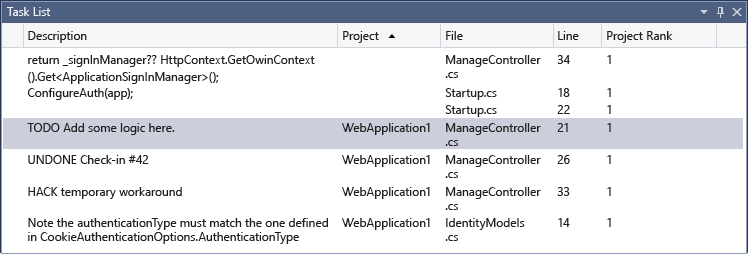
\includegraphics[width=0.9\textwidth]{images/task-list}
\caption{Task List of a modern Integrated Development Environment}
\label{fig:vs-task-list}
\end{figure}
This concept can be applied to the combination of Statecharts and hole-driven development presenting an overview for all currently existing holes.
Due to the additional information provided by holes as described in \cref{chap:possible-applications} this list can be targeted for specific participants in a software project keeping the mental overload as small as possible.
Furthermore instead of showing the file location, the superstate of the hole can be displayed, enhancing the information presented with even more context.
Instead of keeping the tasks to do in mind or using external tools, developers, system analysts, architects and other people in the software development process can be guided by the task list based on the holes in the Statechart in a real single source of truth.


\subsubsection{5\textsuperscript{th} rule: assisting simulation}
As described in \cref{sec:mental-models} the simulation aspect of mental models is fundamental to their applicability.
Statecharts, being a model as well provide this same aspect of simulation.
\cref{fig:xstate-simulation} shows this simulation aspect in practice, the used tool is called XState Visualizer\footnote{\url{}}.
\begin{figure}[h]
\centering
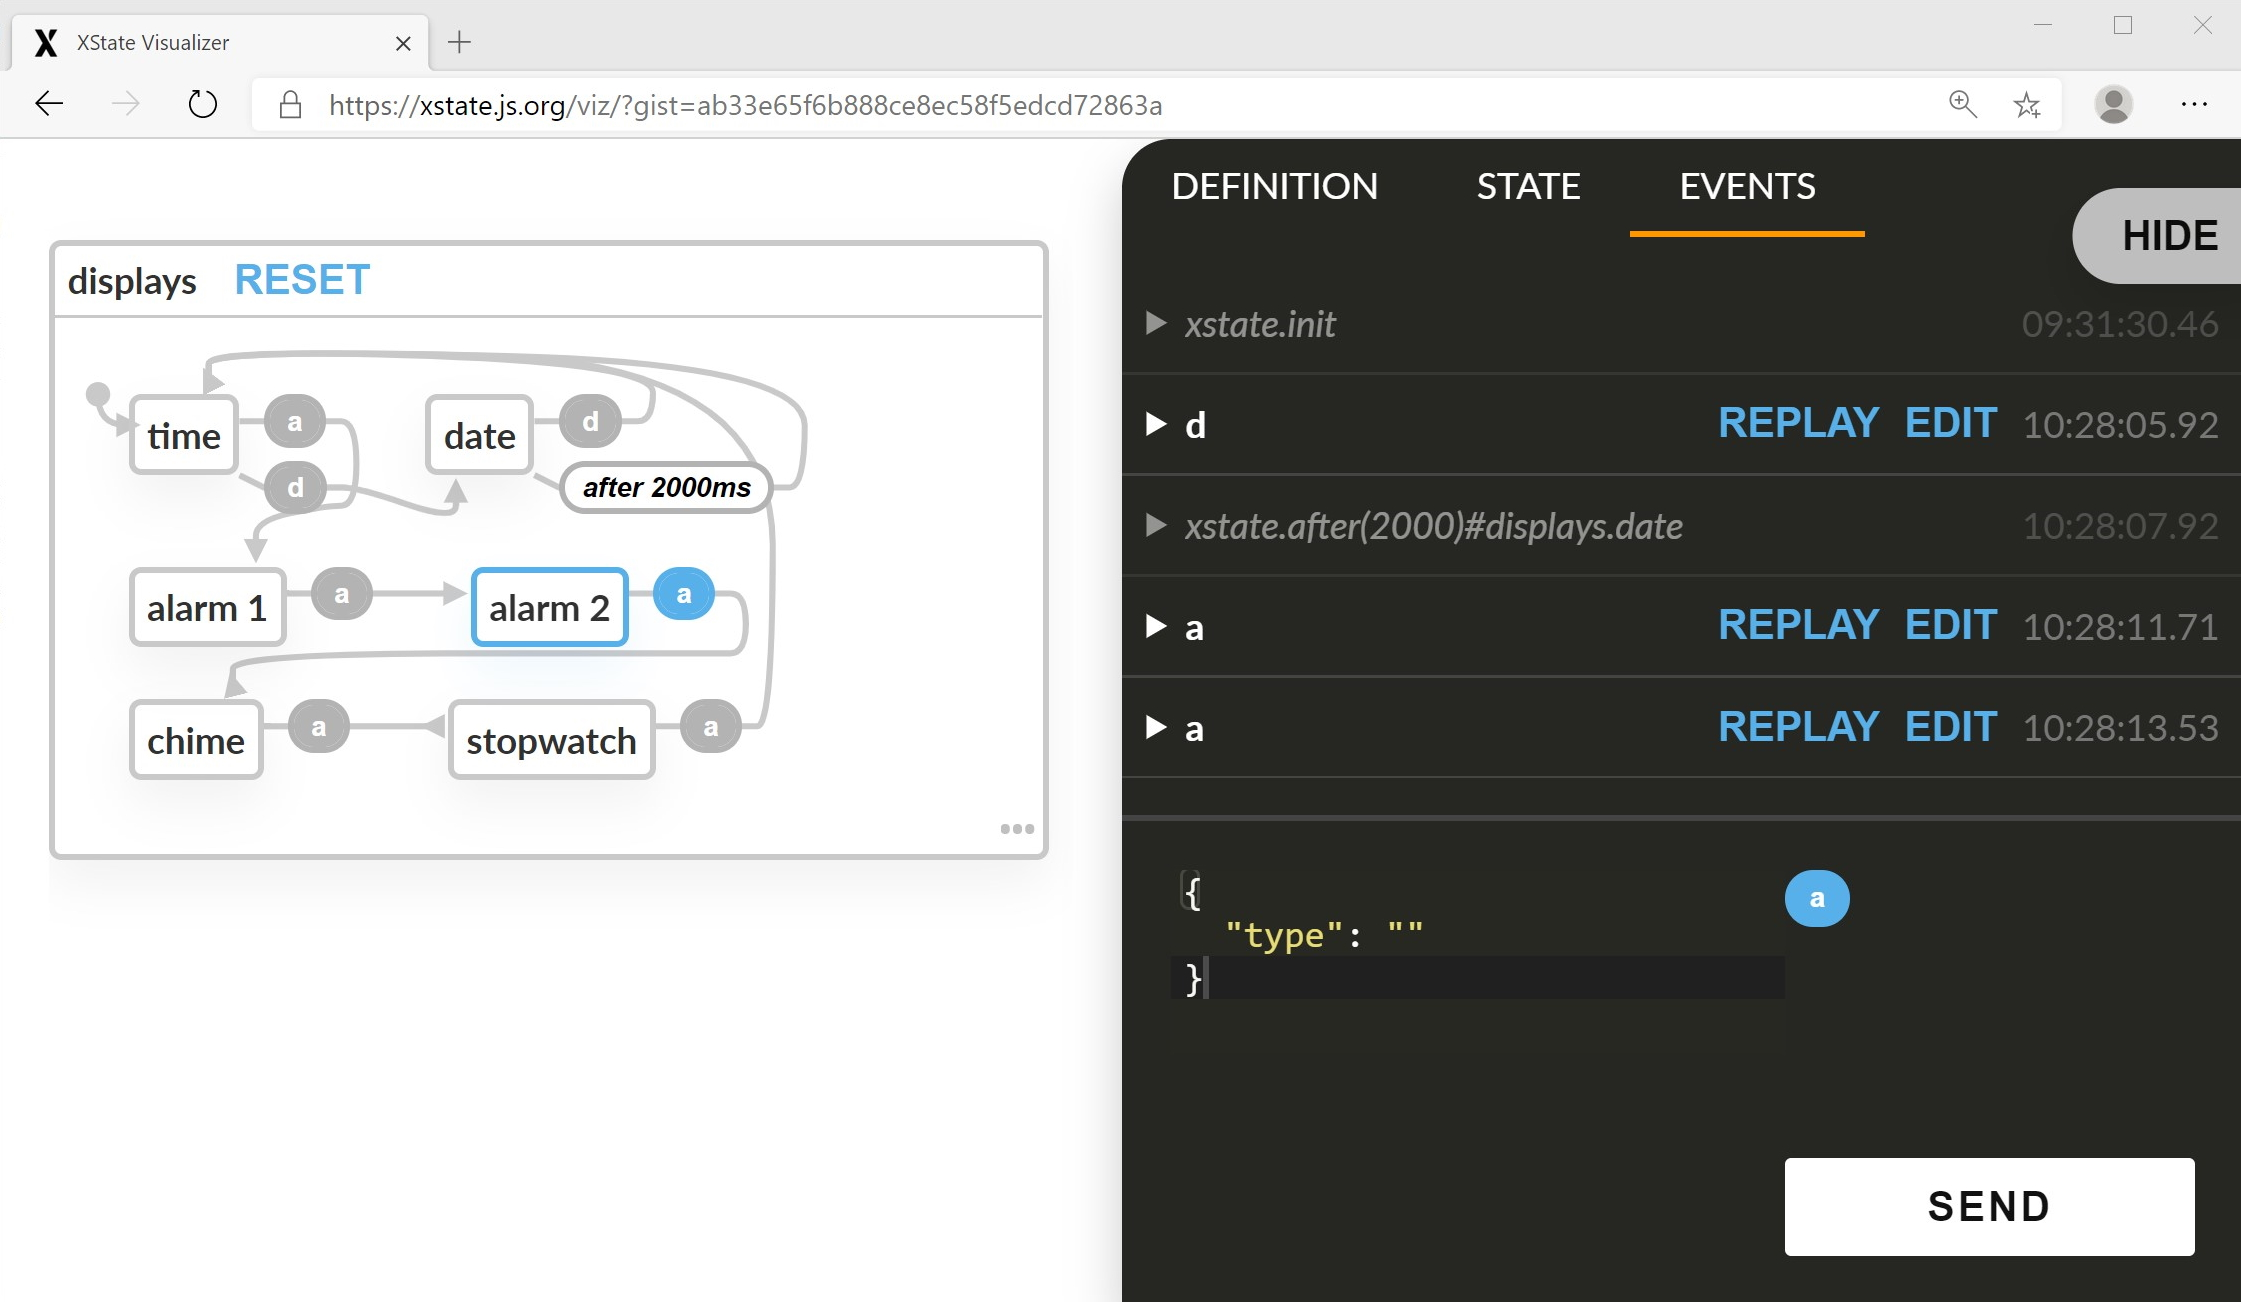
\includegraphics[width=0.9\textwidth]{images/xstate-simulation}
\caption{Simulating Statecharts using the XState Visualizer}
\label{fig:xstate-simulation}
\end{figure}
Despite differences in the notation, the Statechart on the left\footnote{\url{https://xstate.js.org/viz/?gist=ab33e65f6b888ce8ec58f5edcd72863a}} is identical to \cref{fig:statecharts-example}.
On the right side there is an overview of the occurred events over time, the currently active state is highlighted directly in the Statechart.
Events can be raised by clicking on the event names directly in the Statechart.
Looking at the event log one can reconstruct why the currently active state is \emph{alarm 2}.
After initialization the Statechart was in the state \emph{time}. Sending the event \emph{d} sent the Statechart into state \emph{date}, after 2 seconds it transitioned back into \emph{time}.
Sending the event \emph{a} twice, it first transitioned into \emph{alarm 1} and then continued into \emph{alarm 2}.
Creating this mental model of the system, one can simply play around with this interactive visualization immensely reducing the cognitive effort of sharing the underlying mental model \autocite{dutke_mentale_1994}.

% - executability
% - Haskell deferring errors to runtime \verb|-XHoles|